%
% Carátula NO-oficial para 86.22 aboratorio de Control Automático.
%
% Basado en el template realizado por Diego Essaya, disponible en
%                                                         http://lug.fi.uba.ar
% Modificado por Patricio Moreno y Michel Peterson.
% Modificado por Sebastián Santisi.
% Abril 2014: Modificado por Patricio Moreno.
% Septiembre 2017: Modificado por Patricio Moreno.
% Septiembre 2017: Modificado por Ezequiel Pecker Marcosig.

%
% Acá se define el tamaño de letra principal:
% Para utilizar los estilos de KOMA-script, descomentar la línea siguiente y
% comentar la que le sigue (dejar sin comentar un único documentclass)
%\documentclass[10pt]{scrartcl}
\documentclass[10pt]{article}

%
% Título y autor(es):
%
\title{Trabajo Práctico N\b o 2}
\author{CERVETTO, Marcos\\MARCHI, Edgardo\\PECKER MARCOSIG, Ezequiel}

%------------------------- Carga de paquetes ---------------------------
%
% Si no necesitás algún paquete, comentalo.
%

%
% Definición del tamaño de página y los márgenes:
% Si preferís menos márgenes, descomentá la línea anterior
%\usepackage[a4paper,headheight=16pt,scale={0.7,0.8},hoffset=0.5cm]{geometry}

%
% Vamos a escribir en castellano:
%
\usepackage[spanish,es-tabla]{babel}
\usepackage[utf8x]{inputenc}

%
% Para escribir fórmulas matemáticas utilizamos:
%
\usepackage{amsmath}
\usepackage{amssymb}
%
% El paquete amsmath agrega algunas funcionalidades extra a las fórmulas.
% Además defino la numeración de las tablas y figuras al estilo "Figura 2.3",
% en lugar de "Figura 7". (Por lo tanto, aunque no uses fórmulas, si querés
% este tipo de numeración dejá el paquete amsmath descomentado).
%
% \numberwithin{equation}{section}
% \numberwithin{figure}{section}
% \numberwithin{table}{section}

%
% Para tener cabecera y pie de página con un estilo personalizado:
%
\usepackage{fancyhdr}

%
% Para poder controla mejor la poscición de las figuras
%
\usepackage{float}
\usepackage{placeins}
%
% Para poner el texto "Figura X" en negrita:
% (Si no tenés el paquete 'caption2', probá con 'caption').
%
\usepackage[hang,bf]{caption2}

%
% Para poner hipervínculos en el pdf
%
\usepackage[colorlinks=true,linkcolor=black, urlcolor=blue]{hyperref}

%
% Para poder modificar los items de las listas (IEEE style refs.)
%
\usepackage{enumerate}

%
% Para poder usar subfiguras: (al estilo Figura 2.3(b) )
%
%\usepackage{subfig}

%
% Para poder armar tablas con formato
%
\usepackage{booktabs}

%
% Para poder agregar notas al pie en tablas:
%
%\usepackage{threeparttable}

%------------------------------ graphicx ----------------------------------
%
% Para incluir imágenes, el siguiente código carga el paquete graphicx
% según se esté generando un archivo dvi o un pdf (con pdflatex).

% Para generar dvi, descomentá la linea siguiente:
%\usepackage[dvips]{graphicx}

% Para generar pdf, descomentá las dos lineas seguientes:
\usepackage[pdftex]{graphicx}
\pdfcompresslevel=9

%
% Todas las imágenes están en el directorio imgs:
%
\newcommand{\imgdir}{img}
\graphicspath{{\imgdir/}}

\usepackage{subfigure}
%
%------------------------------ graphicx ----------------------------------

% Necesitas este paquete si haces los diagrámas de flujo en el prográma Dia
% y exportás a latex
%\usepackage{tikz}

%------------------------------ color -------------------------------------
% Necesitas este paquete para definir tus propios colores
\usepackage{color}
\definecolor{mygreen}{rgb}{0,0.6,0}
\definecolor{mygray}{rgb}{0.5,0.5,0.5}
\definecolor{mymauve}{rgb}{0.58,0,0.82}
%------------------------------ color -------------------------------------


%----------------------------- listings -----------------------------------
% Necesitas este paquete para mostrar el código.
\usepackage{listings}
\lstdefinestyle{customcpp}{
  backgroundcolor=\color{white},   % choose the background color; you must add \usepackage{color} or \usepackage{xcolor}; should come as last argument
  basicstyle=\small,        % the size of the fonts that are used for the code
  breakatwhitespace=false,         % sets if automatic breaks should only happen at whitespace
  breaklines=true,                 % sets automatic line breaking
  captionpos=b,                    % sets the caption-position to bottom
  commentstyle=\color{mygreen},    % comment style
  deletekeywords={...},            % if you want to delete keywords from the given language
%  escapeinside={\%*}{*)},          % if you want to add LaTeX within your code
  extendedchars=true,              % lets you use non-ASCII characters; for 8-bits encodings only, does not work with UTF-8
  frame=single,	                   % adds a frame around the code
  keepspaces=true,                 % keeps spaces in text, useful for keeping indentation of code (possibly needs columns=flexible)
  keywordstyle=\color{blue},       % keyword style
  language=C++,                 % the language of the code
  morekeywords={*,...},           % if you want to add more keywords to the set
%  numbers=left,                    % where to put the line-numbers; possible values are (none, left, right)
%  numbersep=5pt,                   % how far the line-numbers are from the code
%  numberstyle=\tiny\color{mygray}, % the style that is used for the line-numbers
  rulecolor=\color{black},         % if not set, the frame-color may be changed on line-breaks within not-black text (e.g. comments (green here))
  showspaces=false,                % show spaces everywhere adding particular underscores; it overrides 'showstringspaces'
  showstringspaces=false,          % underline spaces within strings only
  showtabs=false,                  % show tabs within strings adding particular underscores
  stepnumber=2,                    % the step between two line-numbers. If it's 1, each line will be numbered
  stringstyle=\color{mymauve},     % string literal style
  tabsize=2,	                   % sets default tabsize to 2 spaces
  title=\lstname                   % show the filename of files included with \lstinputlisting; also try caption instead of title
}

\lstdefinestyle{custommatlab}{
  backgroundcolor=\color{white},   % choose the background color; you must add \usepackage{color} or \usepackage{xcolor}; should come as last argument
  basicstyle=\small,        % the size of the fonts that are used for the code
  breakatwhitespace=false,         % sets if automatic breaks should only happen at whitespace
  breaklines=true,                 % sets automatic line breaking
  captionpos=b,                    % sets the caption-position to bottom
  commentstyle=\color{mygreen},    % comment style
  deletekeywords={...},            % if you want to delete keywords from the given language
%  escapeinside={\%*}{*)},          % if you want to add LaTeX within your code
  extendedchars=true,              % lets you use non-ASCII characters; for 8-bits encodings only, does not work with UTF-8
  frame=single,	                   % adds a frame around the code
  keepspaces=true,                 % keeps spaces in text, useful for keeping indentation of code (possibly needs columns=flexible)
  keywordstyle=\color{blue},       % keyword style
  language=Matlab,                 % the language of the code
  morekeywords={*,...},           % if you want to add more keywords to the set
%  numbers=left,                    % where to put the line-numbers; possible values are (none, left, right)
%  numbersep=5pt,                   % how far the line-numbers are from the code
%  numberstyle=\tiny\color{mygray}, % the style that is used for the line-numbers
  rulecolor=\color{black},         % if not set, the frame-color may be changed on line-breaks within not-black text (e.g. comments (green here))
  showspaces=false,                % show spaces everywhere adding particular underscores; it overrides 'showstringspaces'
  showstringspaces=false,          % underline spaces within strings only
  showtabs=false,                  % show tabs within strings adding particular underscores
  stepnumber=2,                    % the step between two line-numbers. If it's 1, each line will be numbered
  stringstyle=\color{mymauve},     % string literal style
  tabsize=2,	                   % sets default tabsize to 2 spaces
  title=\lstname                   % show the filename of files included with \lstinputlisting; also try caption instead of title
}
%----------------------------- listings -----------------------------------



%------------------------- Inicio del documento ---------------------------

\begin{document}

%
% Hago que en la cabecera de página se muestre a la derecha la sección,
% y en el pie, en número de página a la derecha:
%
\pagestyle{fancy}
\lhead{\sc TP Nº2 - \sc 2º Cuat. 2017}
\chead{}
\rhead{CERVETTO, MARCHI, PECKER MARCOSIG}
\lfoot{}
\cfoot{}
\rfoot{\thepage}

%
% Carátula:
%
\begin{titlepage}

\thispagestyle{empty}

\begin{center}

\includegraphics[scale=0.3]{img/fiuba}\\
\large{\textsc{Universidad de Buenos Aires}}\\
\large{\textsc{Facultad De Ciencias Exactas y Naturales}}\\
\large{\textsc{Departamento de Computación}}\\
% Modificar año y cuatrimestre
\small{Año 2017 - 2\textsuperscript{do} Cuatrimestre}
\end{center}

\vfill

\begin{center} % Modificar el código de ser necesario
\Large{\underline{\textsc{Simulación de Eventos Discretos}}}
\end{center}

\vfill

\begin{tabbing}
\hspace{2cm}\=\+TRABAJO PRÁCTICO Nº \textless{}2\textgreater{}\\
	TEMA:\textless{}Manejo del Inventario de una Industria\textgreater{}\\
	FECHA:\textless{\today}\textgreater{}\\
\\
	INTEGRANTES:\hspace{-1cm}\=\+\hspace{1cm}\=\hspace{6cm}\=\\
		CERVETTO, Marcos	\>\>- \#FIUBA\\
			\>\footnotesize{\verb!<cervettomarcos@gmail.com>!}\\
		MARCHI, Marcos	\>\>- \#FIUBA\\
			\>\footnotesize{\verb!<edgardo.marchi@gmail.com>!}\\
		PECKER MARCOSIG, Ezequiel	\>\>- \#FIUBA\\
			\>\footnotesize{\verb!<ezepecker@gmail.com>!}\\
\end{tabbing}

\vfill

\hrule
\vspace{0.2cm}

% Modificar código de ser necesario
\noindent\small{Simulación de Eventos Discretos}

\end{titlepage}

%
% Hago que las páginas se comiencen a contar a partir de aquí:
%
\setcounter{page}{1}

%
% Pongo el índice en una página aparte:
%
\tableofcontents
\newpage

%
% Inicio del TP:
%

\section{Objetivo y Enunciado}
%El objetivo de este Trabajo Práctico es demostrar la comprensión del modelado y simulación utilizando el formalismo DEVS, junto a la aplicación de las técnicas mediante la herramienta CD++.
%Se deberá identificar un sistema del mundo real que pueda ser representado usando DEVS y construir luego un modelo del mismo.
%Finalmente se ejecutarán simulaciones del sistema analizado. El sistema estudiado puede ser natural o artificial, y puede existir en la realidad o no.

\section{Modelo Conceptual}
\subsection{Motivación\label{sec:motivacion}}

Una compañía que vende un único producto está interesada en estudiar la forma óptima de ordenamiento de las unidades producidas en el almacén.

En la Figura \ref{fig:esquema-del-problema} se muestra un esquema de la industria, donde se observa la ubicación del inventario.

Para este trabajo, el bloque Inventario se va a modelizar con autómata celular.

\begin{figure}[h]
\centering
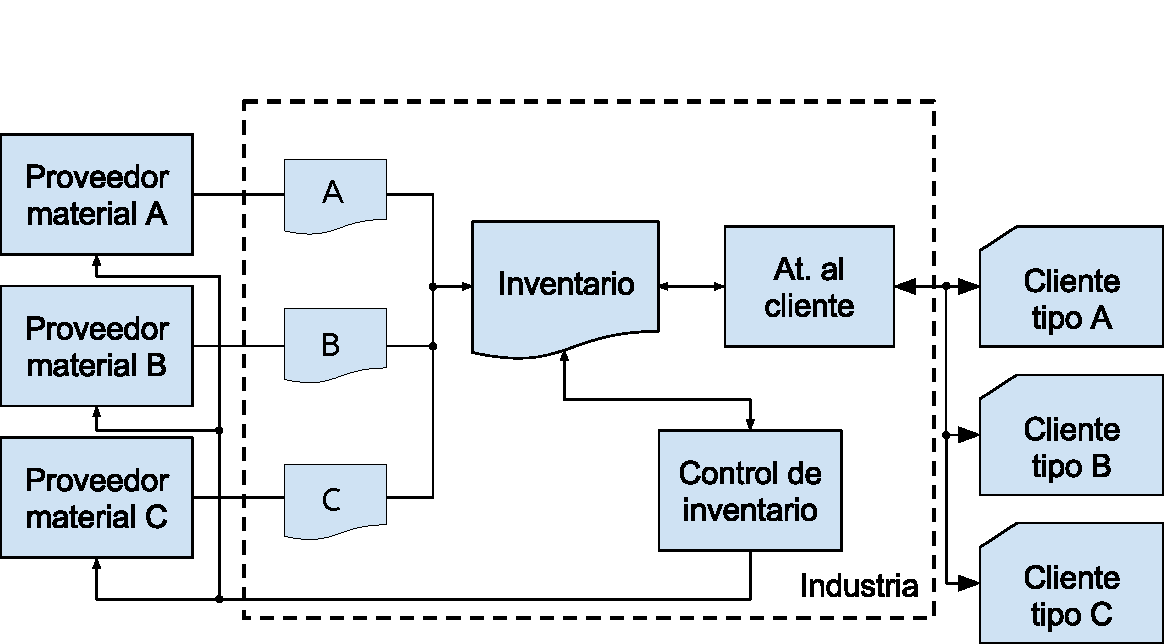
\includegraphics[width=\textwidth]{img/figura1}
\caption{Esquema del problema planteado.}
\label{fig:esquema-del-problema}
\end{figure}
\FloatBarrier 

\subsection{Autómata Celular\label{sec:AC}} 

 El bloque atómico DEVS correspondiente al Inventario que se indica en la Figura \ref{fig:esquema-del-problema} va a ser reemplazado por tres bloques cell-DEVS, según la Figura \ref{fig:AC-esquematico}.
 
 \begin{figure}[h] 
 	\centering
 	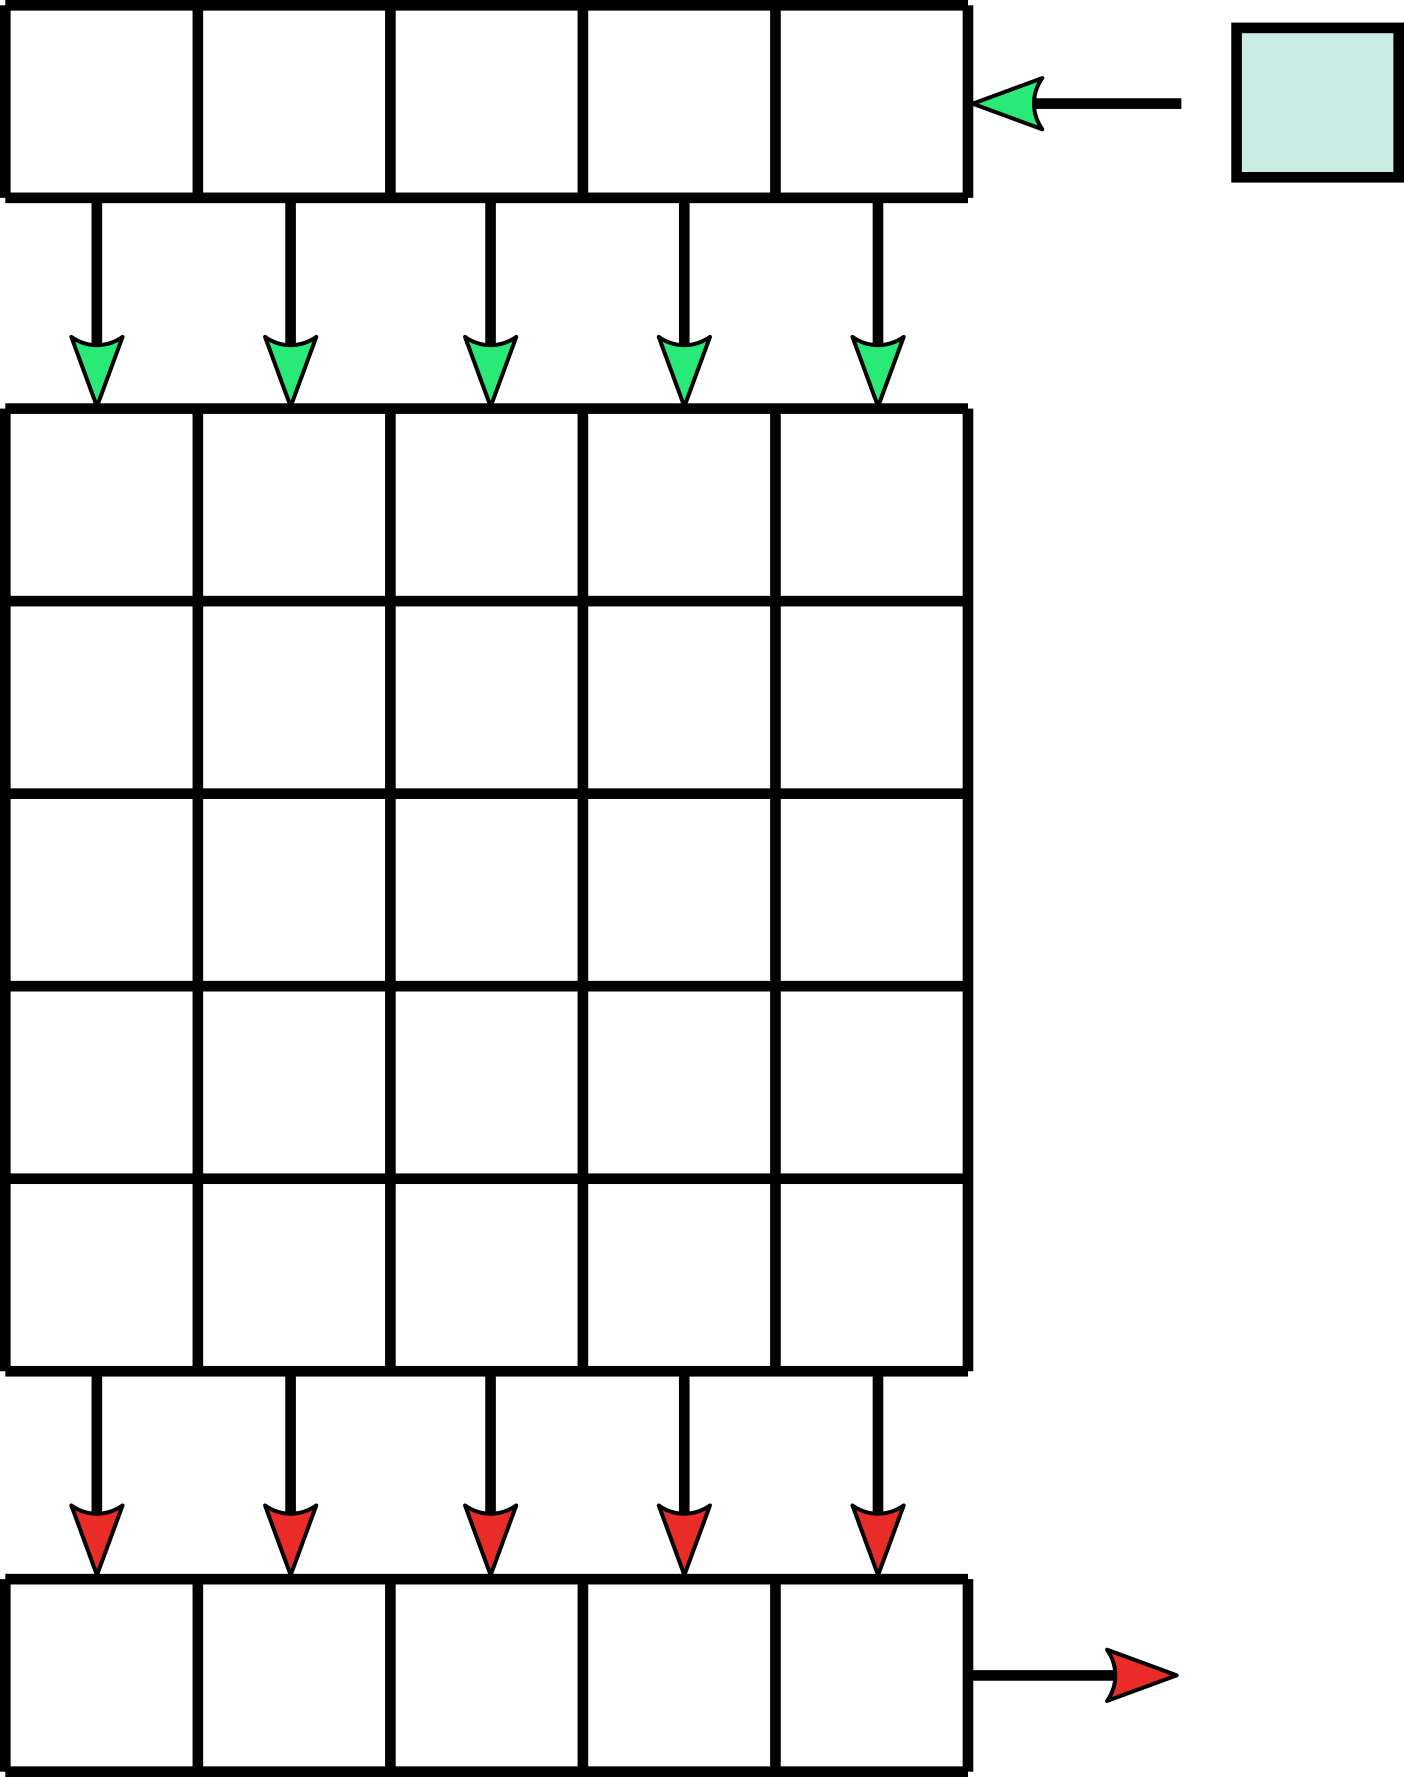
\includegraphics[width=0.5\textwidth]{grilla} 
 	\caption{Inventario con cell-DEVS.} 
 	\label{fig:AC-esquematico} 
 \end{figure}
 \FloatBarrier
 
 El primer bloque corresponde a una fila de celdas que manejarán la ubicación inicial de los productos dentro del inventario. Del trabajo 1 se puede recordar que cada producto tiene una fecha de vencimiento asociada. Esta fecha será la que determine la columna en la que se apilará a cada producto. Por ejemplo: si falta menos de una semana para su vencimiento se apilará en la columna 0 (más a la derecha), si falta entre 1 y 2 semanas en la columna 1, entre 2 y 3 en la columna 2, etc. Este proceso se esquematiza en la Figura \ref{fig:AC-ingreso-de-productos}.
 
 \begin{figure}[h] 
 	\centering 
 	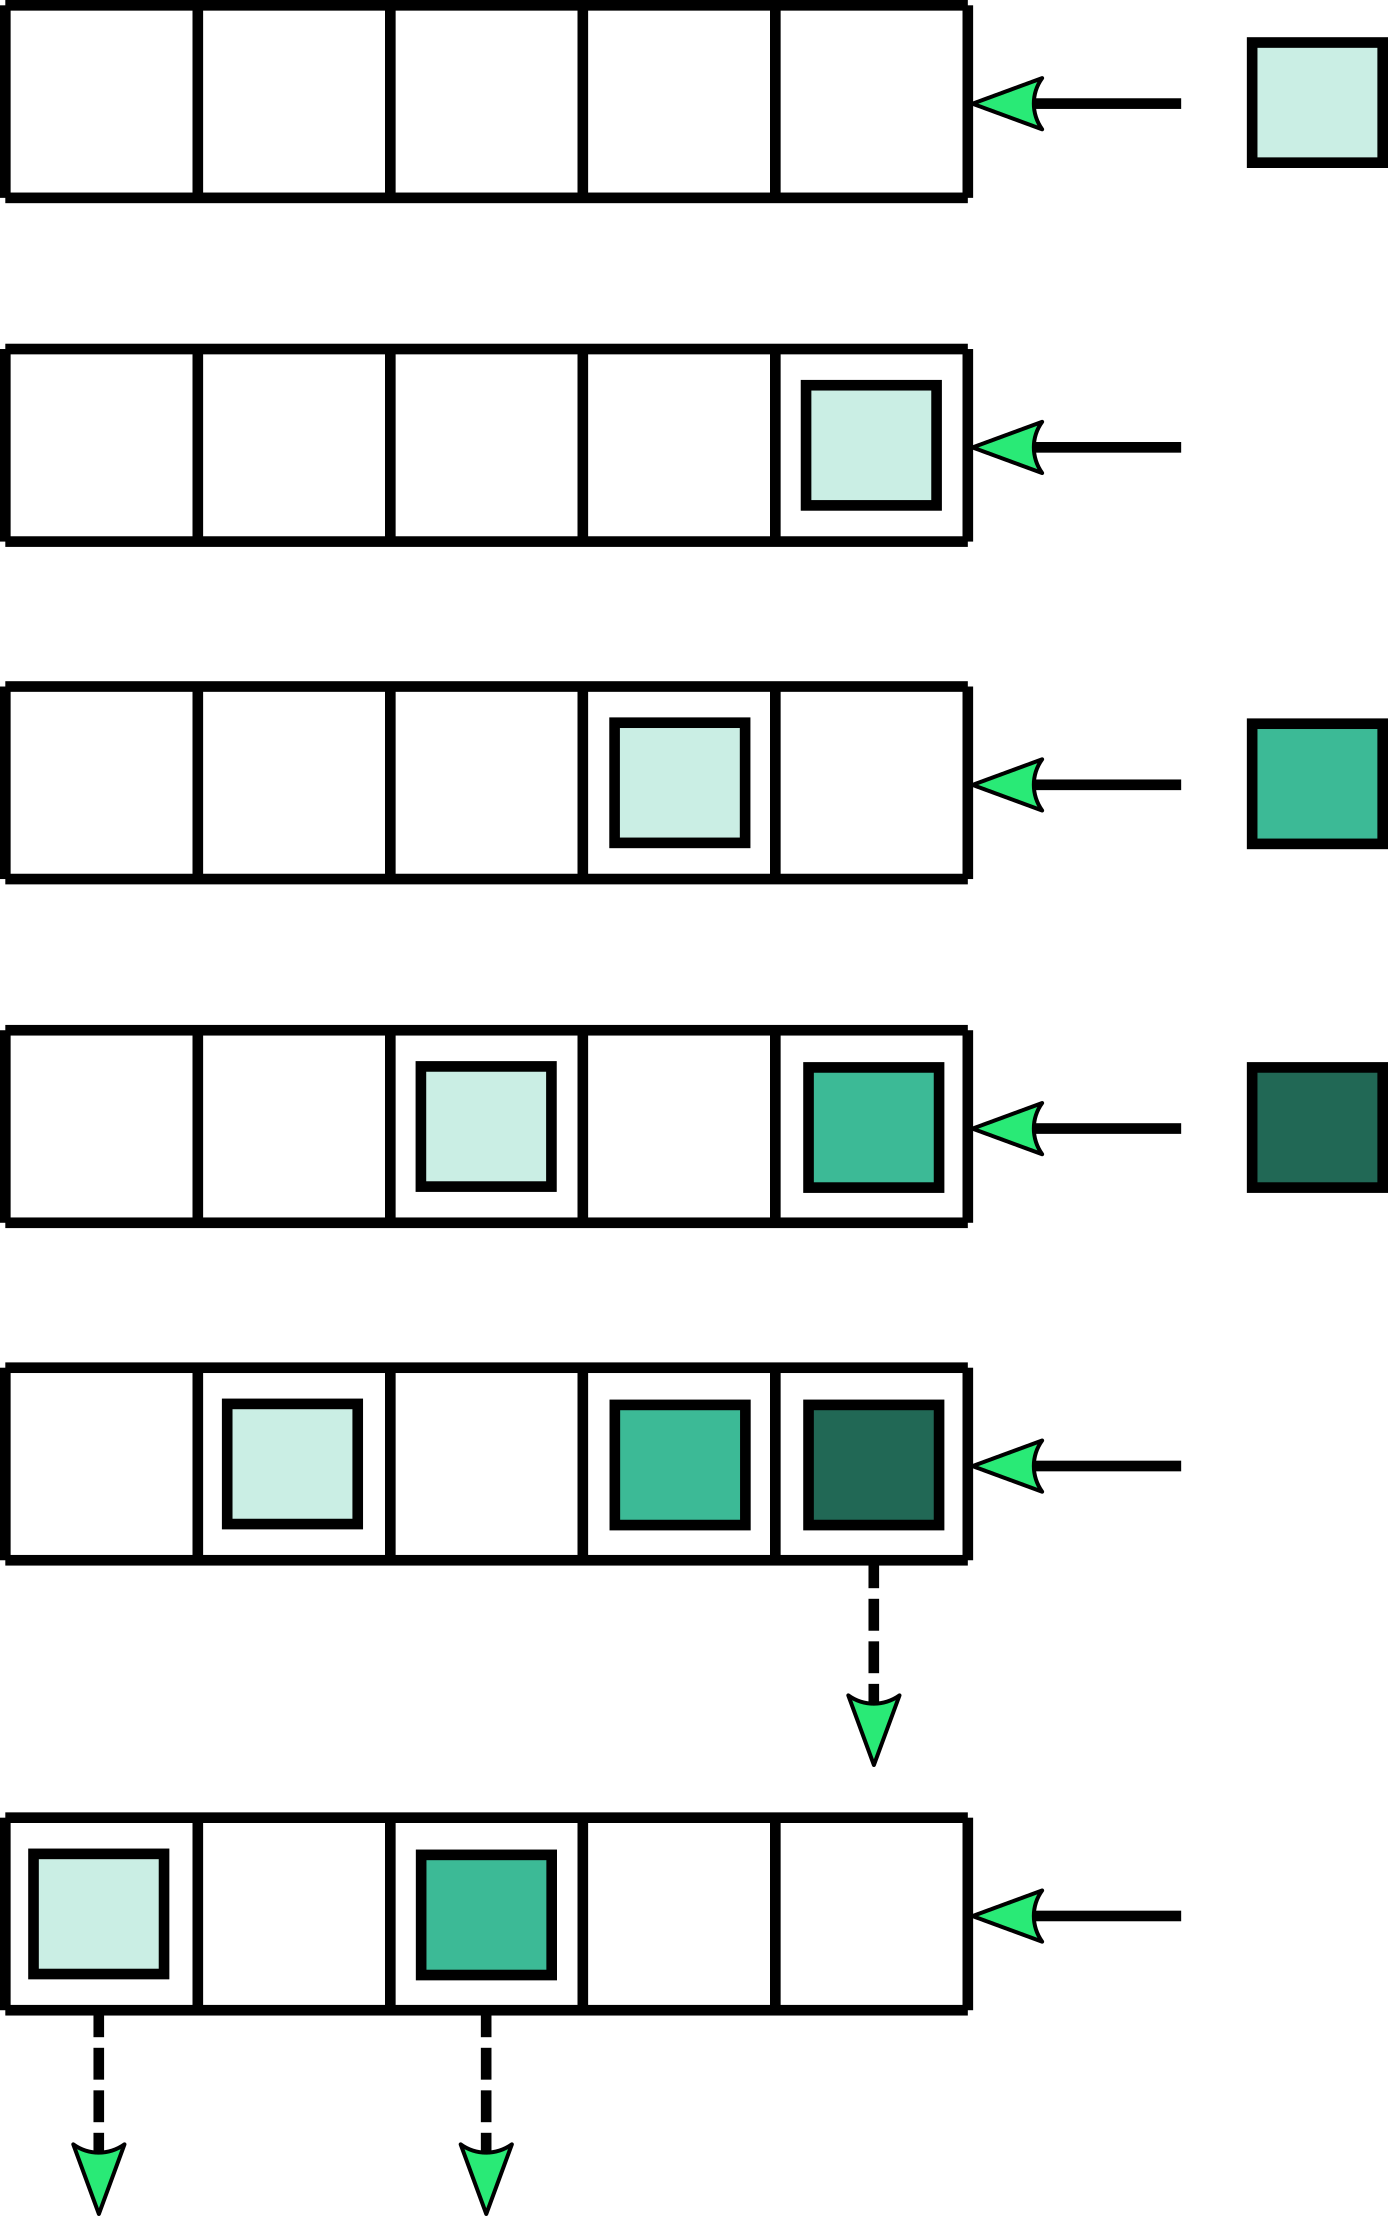
\includegraphics[width=0.5\textwidth]{entrada} 
 	\caption{Ingreso de productos al inventario.} 
 	\label{fig:AC-ingreso-de-productos} 
 \end{figure}
 \FloatBarrier
 
 El segundo bloque será el inventario propiamente dicho. Es una grilla donde las columnas representan posiciones de apilamiento de productos. Las entradas de productos se realizan por la parte superior de cada columna, de forma de ir apilándolos. La salida de productos se realiza por la parte inferior de cada columna. Periódicamente se chequea la fecha de vencimiento de cada producto, y si cumple la condición de la columna siguiente a la derecha, por ejemplo que falte menos de N semanas para que perezca, el producto se intenta mover a esa columna.
 
 La salida de productos está físicamente cercana a la columna derecha (la que contiene a los productos más próximos a vencer). El encargado de retirar productos demora un tiempo hasta llegar a la columna N por lo que idealmente se prefiere retirar los productos de la columna 0. Sin embargo si no hay productos con una fecha de vencimiento tan próxima, deberá recorrer las columnas hasta llegar a un producto. Este proceso de retiro de elementos se modela con el tercer bloque cell-DEVS, en este caso también de una sola fila.
 Todo este proceso se puede observar en la figura en la Figura \ref{fig:AC-inventario}. La fecha de vencimiento se grafica según el esquema de colores de la Figura \ref{fig:AC-colores}.
 
 \begin{figure}[h] 
 	\centering 
 	
\includegraphics[width=0.3\textwidth]{colores} 
 	\caption{Codificación de colores por fecha de vencimiento.} 
 	\label{fig:AC-colores} 
 \end{figure}
 
 \begin{figure}[h] 
 \centering
 
 	\begin{tabular}{cc}
 		\multicolumn{2}{c}{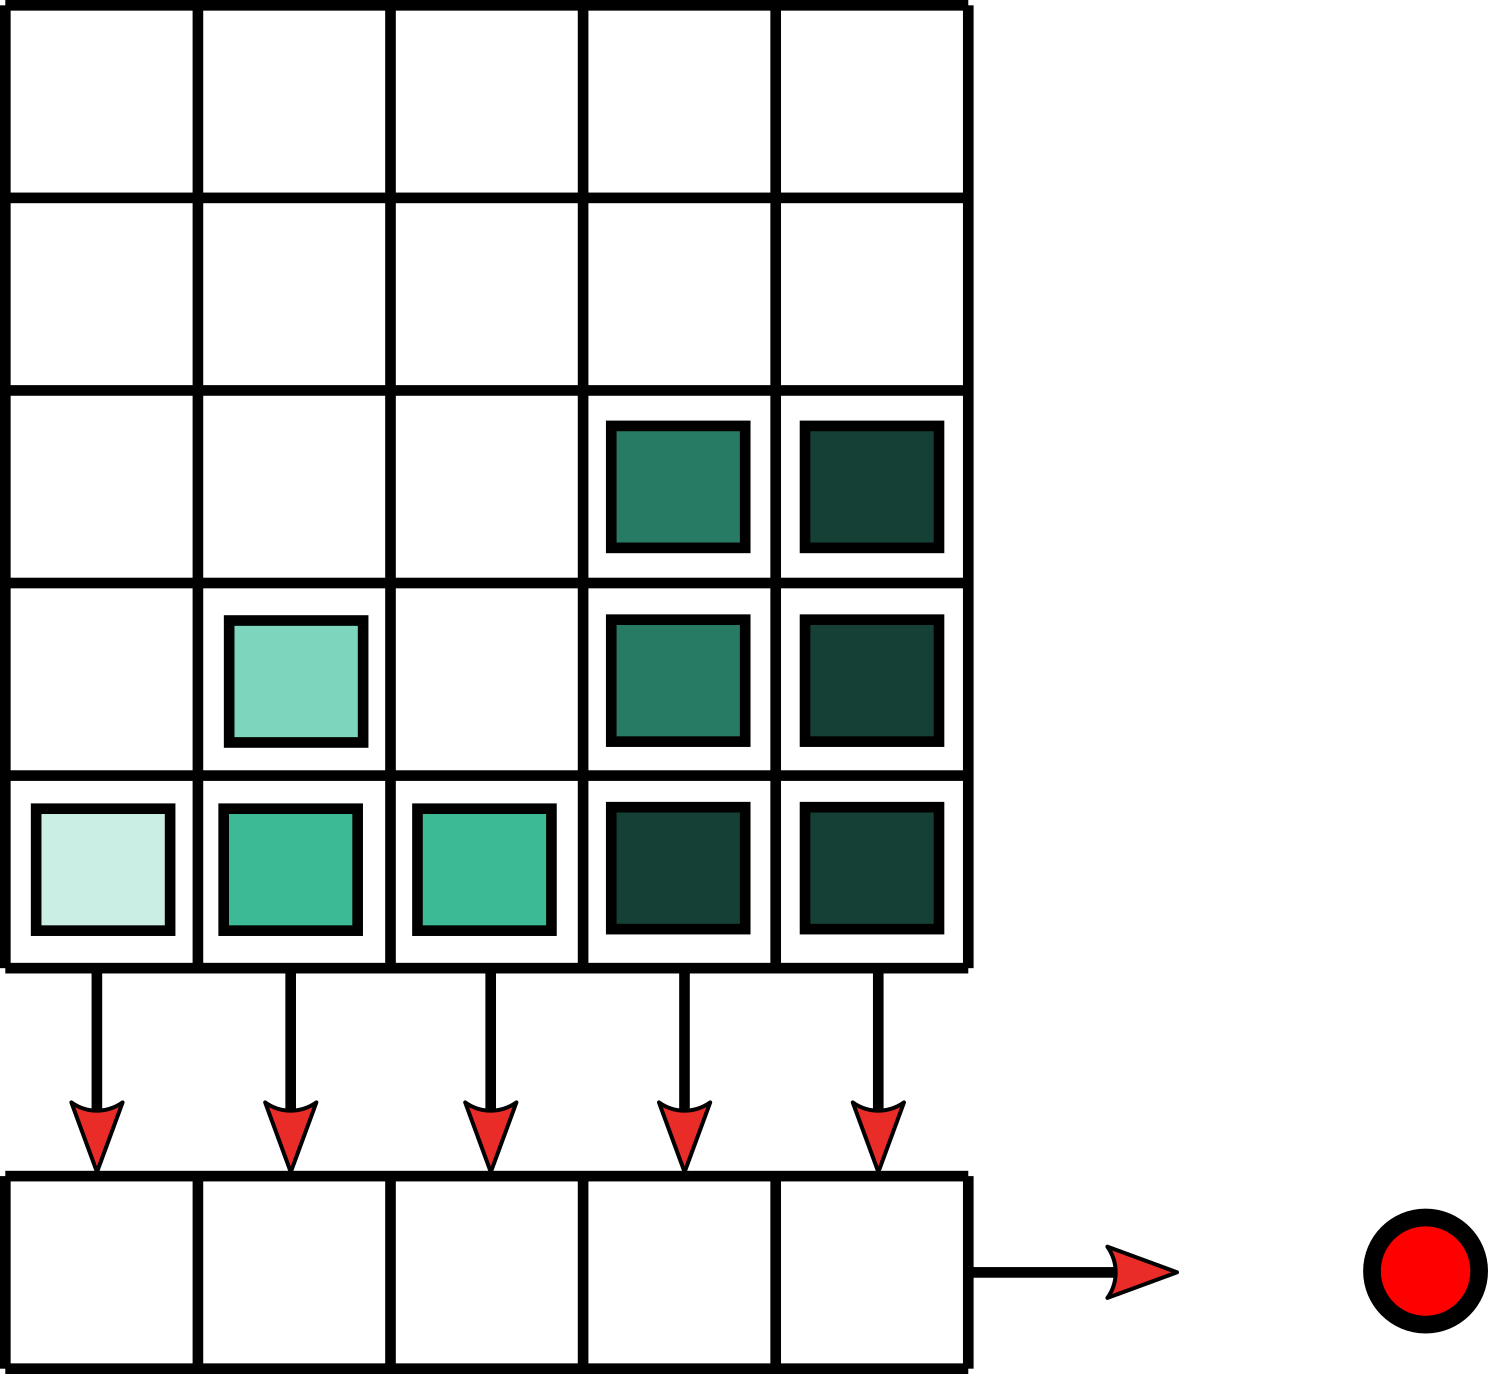
\includegraphics[width=0.4\linewidth]{pedido1}}\\[5mm]
 		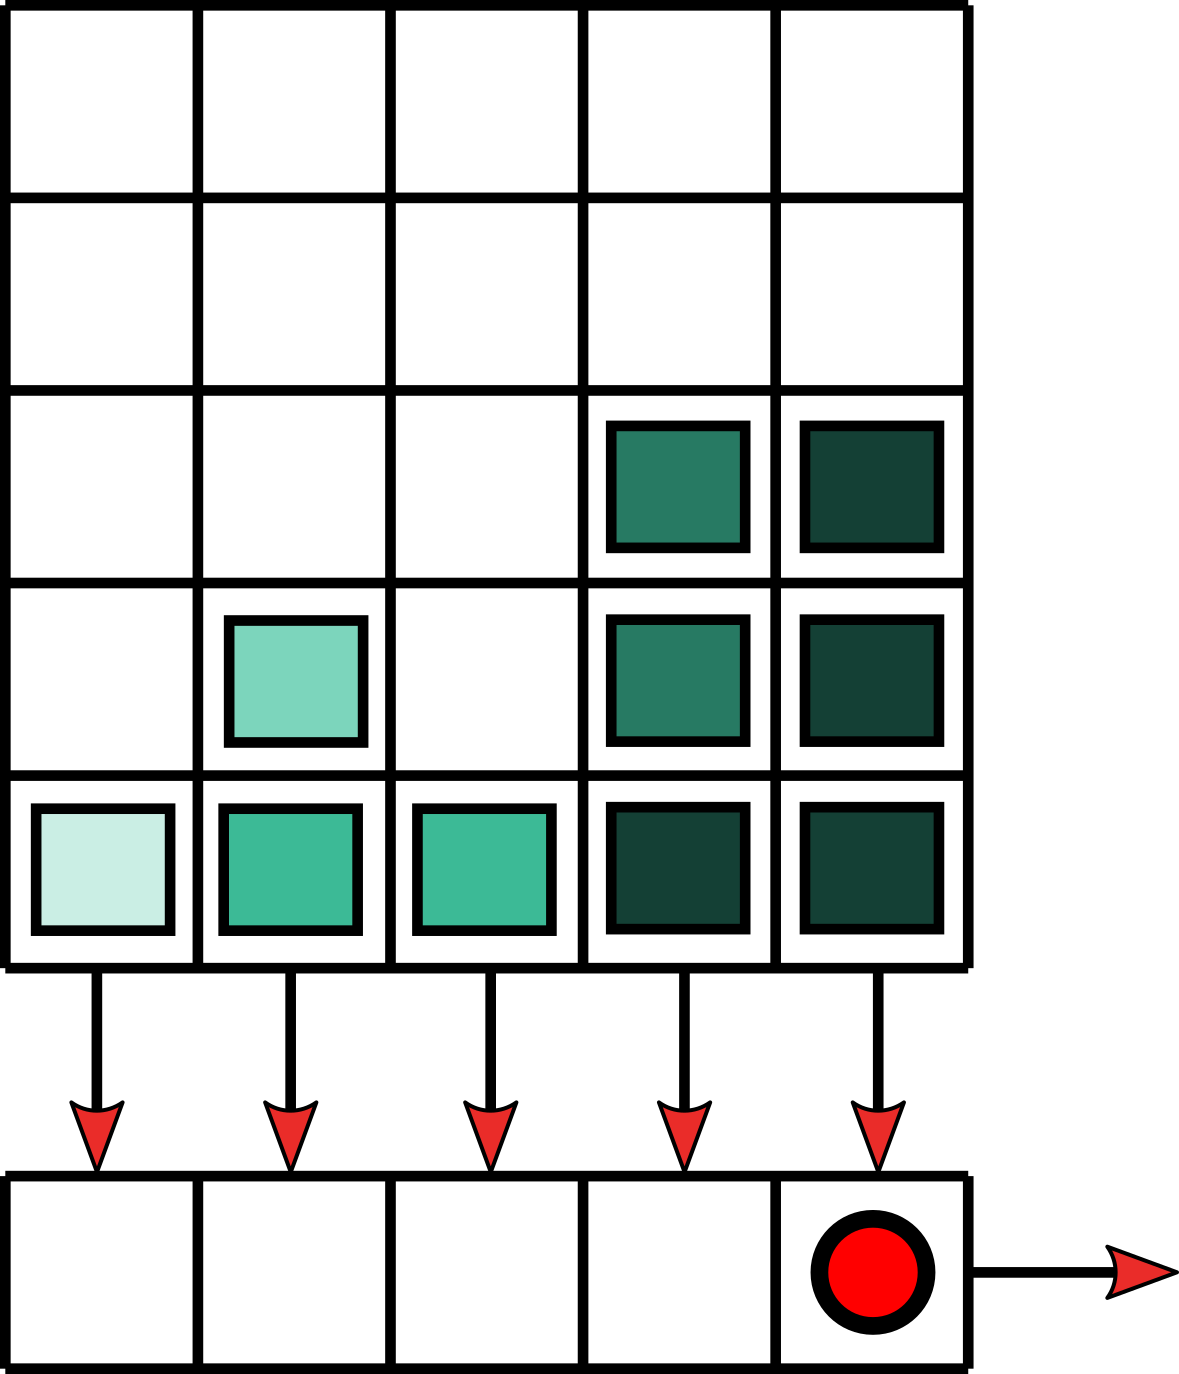
\includegraphics[width=0.3\linewidth]{pedido2} &
 		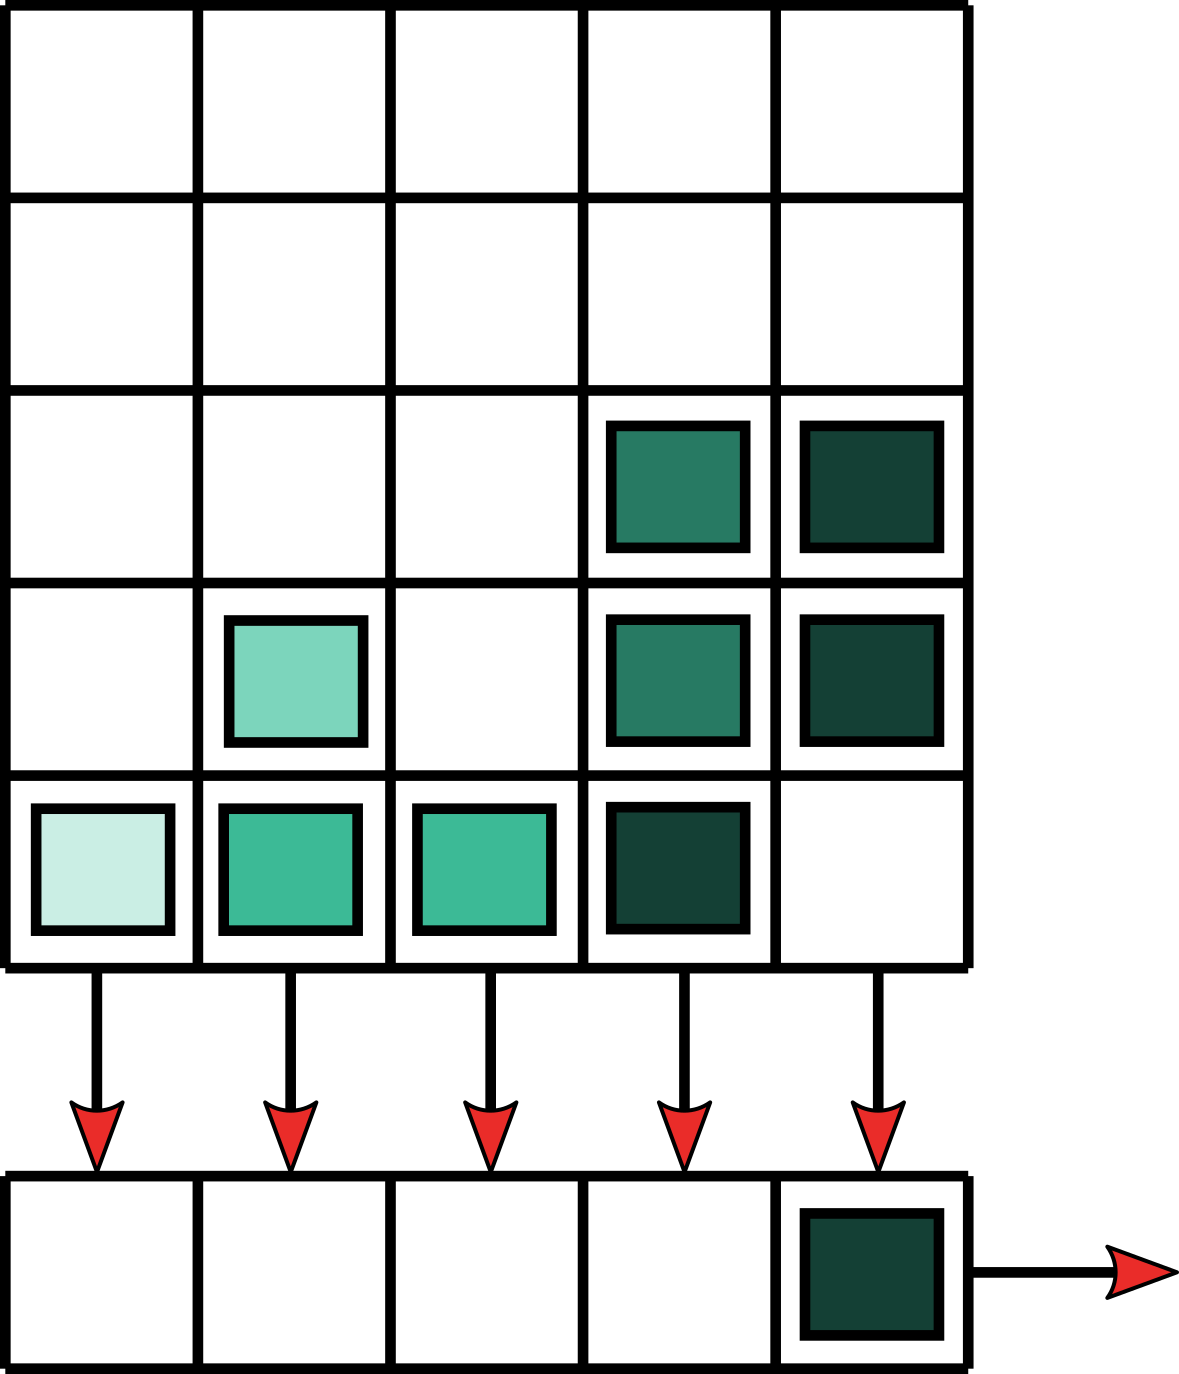
\includegraphics[width=0.3\linewidth]{pedido3} \\[5mm]
 		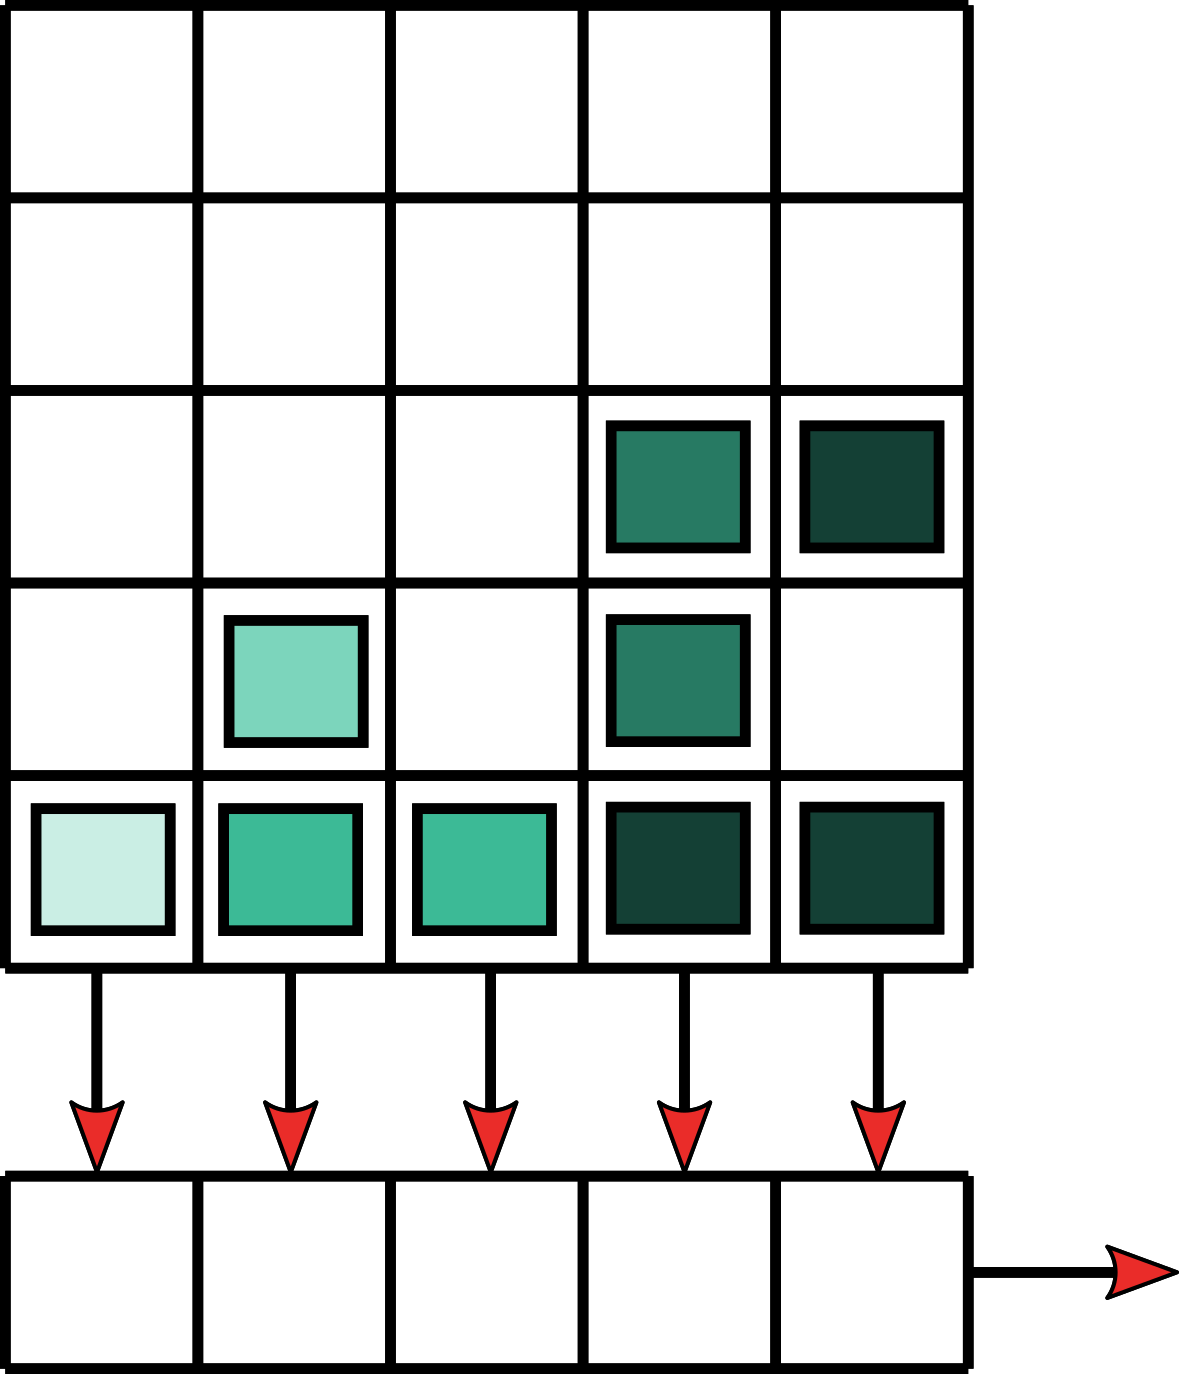
\includegraphics[width=0.3\linewidth]{pedido4} &
 		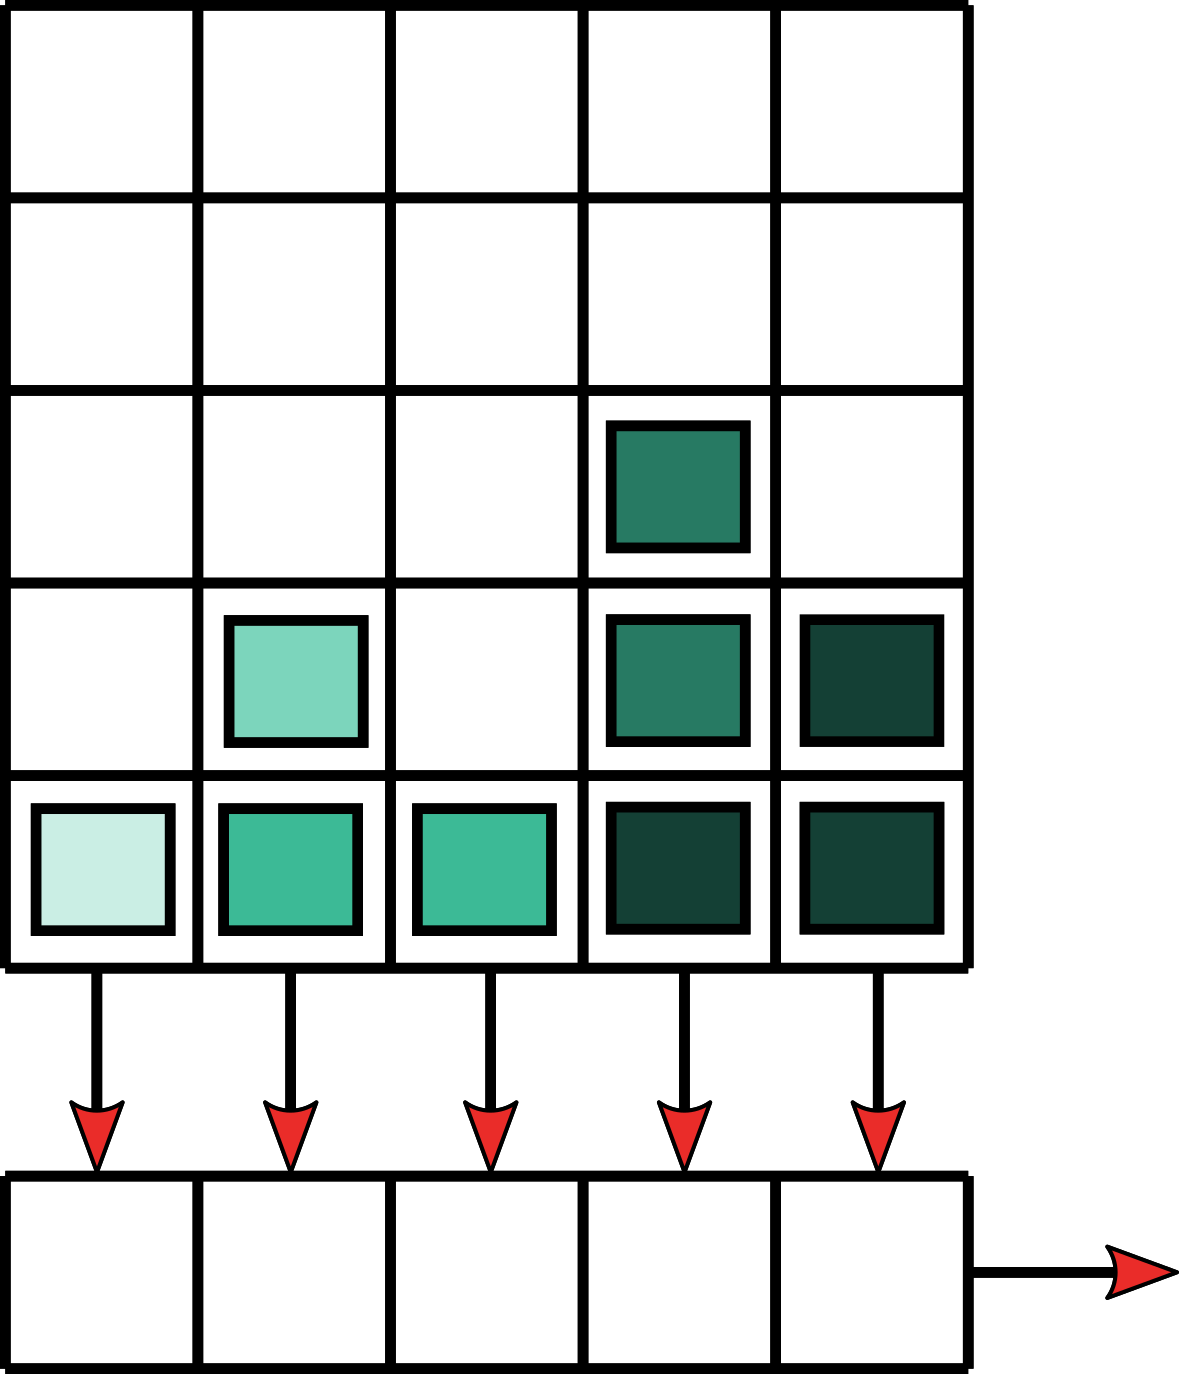
\includegraphics[width=0.3\linewidth]{pedido5} \\
 	\end{tabular}
 	
 	\caption{Autómata celular del inventario.} 
 	\label{fig:AC-inventario} 
 \end{figure}
 \FloatBarrier
 
\subsection{Celdas}

El objetivo del autómata celular es ordenar los productos en el almacén de modo que aquellos con fecha de vencimiento más próxima queden ubicados espacialmente más cerca de la salida, de modo de ser despachados más rápido. De esta manera se busca reducir la cantidad de productos vencidos dentro del almacén. Para esto, periódicamente se revisan las fechas de vencimiento de los productos estampadas en un código de barras en cada unidad. Su ubicación depende del valor de su fecha de vencimiento. Los productos sólo pueden ser movidos si la columna adyacente a la derecha tiene una ubicación disponible hasta un nivel por encima de la altura de ubicación del producto.
Cabe destacar que si la ubicación inferior a donde se encuentra un producto está libre, el producto baja hasta estar apoyado sobre otro producto o sobre el suelo del depósito.
Por estos motivos (y por la preferencia de movimiento hacia la derecha) el vecindario propuesto se puede ver en la Figura~\ref{fig:AC-vecindario}.

\begin{figure}[h] 
  \centering 
  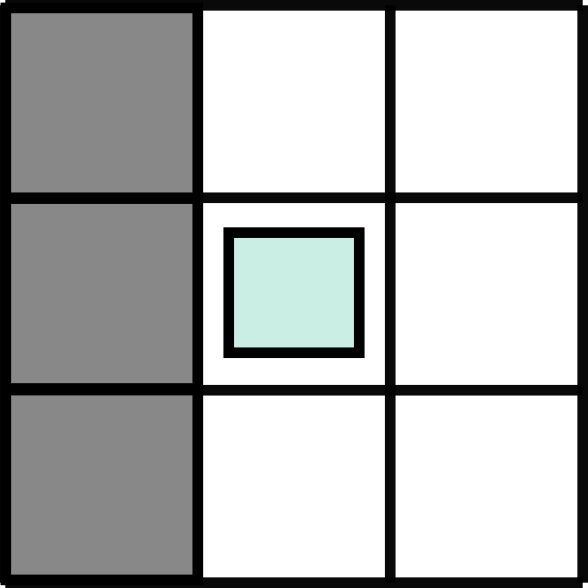
\includegraphics[width=0.3\textwidth]{vecindario} 
  \caption{Vecindario.} 
  \label{fig:AC-vecindario} 
\end{figure}
\FloatBarrier

Las preguntas a responder mediante simulaciones son:
\begin{itemize}
\item \textit{¿Qué política de ordenamiento es óptima para minimizar la cantidad de unidades vencidas al momento del despacho?}
\item Y conectada con la pregunta anterior, \textit{¿qué política de ordenamiento permite minimizar el tiempo necesario para despachar una unidad?}
\end{itemize}
% \FloatBarrier


\appendix
\section{Código Implementado}

\url{https://github.com/TwinT/DEVS-Inventario}

% Please don't exchange the bibliographystyle style
\bibliographystyle{IEEEtran.bst}
% AUTHOR: Include your bib file here
\bibliography{IEEEexample}

\end{document}

